\documentclass[convert={outext=.svg,density=750}]{standalone}
\usepackage{amsmath}

% More defined colors
\usepackage[dvipsnames]{xcolor}

% Required package
\usepackage{tikz}
\usetikzlibrary{positioning}
\usetikzlibrary{shapes.multipart}


\begin{document}

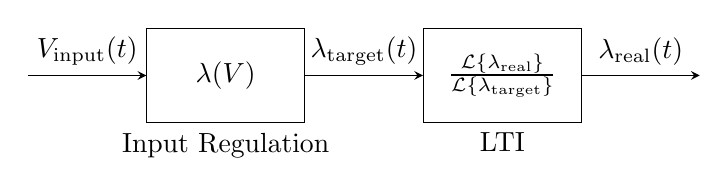
\begin{tikzpicture}[every text node part/.style={align=center}]
    % Input regulation
    \node [draw,
        minimum width=2cm,
        minimum height=1.2cm,
        label=below:Input Regulation
    ]  (input_regulation) at (0,0){$\lambda(V)$};

    % Wavelength Conversion
    \node [draw,
        minimum width=2cm,
        minimum height=1.2cm,
        label=below:LTI,
        right=1.5cm of input_regulation,
    ]  (LTI){$\frac{\mathcal{L}\{\lambda_\text{real}\}}{\mathcal{L}\{\lambda_\text{target}\}}$};

    % Arrows
    \node (foo)[left of=input_regulation]{};
    \draw[stealth-] (input_regulation.west) -- ++(-1.5,0)
    node[midway,above](){$V_\text{input}(t)$};

    \draw[-stealth] (input_regulation.east) -- (LTI.west)
    node[midway,above](){$\lambda_\text{target}(t)$};

    \draw[-stealth] (LTI.east) -- ++(1.5,0)
    node[midway,above](){$\lambda_\text{real}(t)$};


\end{tikzpicture}

\end{document}
